\documentclass[12pt]{article}
\usepackage{hyperref}
\usepackage{graphicx}
\usepackage{amsmath}
\usepackage{listings}
\usepackage{url}
\usepackage{tikz}
\usetikzlibrary{positioning}

\title{Loreum: AI-Powered Decentralized Governance}
\author{Chad Lynch \\ \small{chad@loreum.org} \\ \small{version: 0.1.2}}
\date{\today}

\begin{document}

\maketitle

\begin{abstract}
Loreum is a Smart Account framework that integrates artificial intelligence agents with decentralized capital management and directorship. By combining AI agents with on-chain smart contract systems, Loreum addresses fundamental limitations in traditional corporate and DAO governance structures. The system introduces a novel Chamber architecture that enables dynamic, market-driven governance while maintaining human oversight through a unique delegation mechanism.
\end{abstract}

\section{Introduction}
Traditional organizational governance faces significant challenges in coordination efficiency and decision-making processes. These limitations are particularly evident in decentralized autonomous organizations (DAOs), where governance often becomes bottlenecked by human coordination challenges. Loreum addresses these limitations by introducing an AI-enhanced governance framework that maintains human oversight while leveraging algorithmic precision in decision-making.

\section{System Architecture}

\subsection{Chamber Design}
The Chamber represents a novel smart account architecture that fundamentally reimagines organizational governance through three integrated components: board management, wallet operations, and delegation mechanics. At its core, the system maintains a doubly-linked list structure that tracks delegated voting power and automatically maintains an ordered ranking of leaders. This structure interfaces with a multi-signature wallet system that enforces collective decision-making through quorum requirements.

The security model for AI agent integration relies on market-driven delegation weights combined with strict consensus requirements. All transactions within the system require approval from a minimum of 51\% of the current board, with board positions themselves being determined by the relative weight of delegated tokens. This creates a dynamic security layer where voting power can be rapidly reallocated in response to agent behavior or performance.

\subsection{Market-Driven Governance}
The Chamber implements a futarchic governance model through its delegation mechanism, creating a continuous market for leadership positions. Token holders can delegate their governance power to any NFT ID within the system, with these delegations being tracked through a sophisticated double-entry bookkeeping system. The delegation weights determine leadership positions in real-time, with the top N positions by weight receiving director status and associated transaction approval rights.

This market-driven approach creates natural selection pressure for effective leadership, as token holders can fluidly reallocate their delegation in response to performance. The system maintains atomic consistency through reentrancy protection and ensures that all delegated power can be withdrawn immediately if needed, creating a responsive governance mechanism that can rapidly adapt to changing conditions.

\subsection{Technical Implementation}
The Chamber's core functionality is implemented through a sophisticated combination of data structures and consensus mechanisms. The board structure utilizes a doubly-linked list that maintains nodes containing tokenId, amount, and positional data. This structure enables O(n) insertion and removal operations while maintaining a constantly sorted order of delegations. The system implements automatic reordering on delegation changes, ensuring that the leadership structure always reflects current market sentiment.

The wallet operations layer implements a multi-signature system with batch transaction support, enabling efficient operations while maintaining security through distributed consensus. Transaction execution requires explicit confirmation from a quorum of directors, with all confirmations being revocable until execution. This creates a flexible yet secure framework for treasury management and organizational operations.

\subsection{Security Architecture}
The security model implements multiple complementary layers of protection. Access control is managed through a combination of on-chain validation of board membership and dynamic quorum calculations based on the current board size. All state-changing operations are protected by reentrancy guards, preventing potential attack vectors during complex transaction sequences.

Transaction safety is ensured through a multi-signature requirement that enforces collective decision-making. The system requires confirmation from a threshold of 51\% of board seats before any transaction can be executed, with all confirmations being revocable until execution. This creates a time window for detection and prevention of potentially malicious transactions while maintaining operational efficiency through batch execution support.

The delegation security layer implements comprehensive validation of all token movements and maintains strict accounting of delegated amounts. The system enforces atomic operations for all delegation changes and implements immediate withdrawal capabilities, ensuring that token holders maintain ultimate control over their delegated power. This creates a robust foundation for integrating AI agents while maintaining human oversight through market mechanisms.

\subsection{Token Economics}
The system implements a carefully designed dual-token model that separates governance power from identity:

\begin{enumerate}
    \item Governance Token (ERC20)
    The fungible governance token serves as the primary mechanism for allocating and delegating voting power within the system. Token holders can delegate their voting power to leaders they trust, creating a market-driven approach to governance where the most effective leaders naturally accumulate more influence. This creates strong incentives for responsible leadership and active participation in governance.
    
    \item Identity Token (ERC721)
    Non-fungible tokens are used to establish unique identities for both human participants and AI agents within the system. These tokens serve as the targets for delegation, allowing governance power to flow to specific entities. The NFTs also enable precise tracking of leadership positions and voting power accumulation, providing transparency into the governance structure.
\end{enumerate}

\section{AI Agent Integration}

\subsection{Agent Capabilities}
The AI agents integrated into the Chamber framework perform several critical functions that enhance governance efficiency and security. They continuously analyze on-chain data to provide insights for treasury management decisions, including asset allocation and risk assessment. The agents implement sophisticated monitoring systems to detect and flag suspicious transactions or unusual patterns that may indicate security threats. Through analysis of historical governance data and current market conditions, they generate data-driven insights to inform decision-making processes. For routine operational matters, the agents can execute automated decisions within carefully defined parameters. In more complex scenarios, they facilitate collaboration between human leaders by providing analysis, generating proposals, and modeling potential outcomes.

\subsection{Safety Mechanisms}
The system incorporates multiple layers of safety mechanisms to ensure responsible operation. Human oversight is maintained through a delegation system that allows token holders to quickly withdraw support from underperforming or malicious agents. All delegated authority can be revoked through token withdrawal, providing an immediate check on agent power. The agents operate within clearly defined operational parameters that limit their autonomy and prevent unexpected behavior. Comprehensive performance monitoring systems track agent actions and outcomes, enabling rapid detection and response to any anomalies.

\section{Governance Mechanism}

\subsection{Leadership Structure}
The Chamber implements an innovative leaderboard system that dynamically adjusts to changing delegation patterns. Token holders can delegate their voting power to specific NFT IDs, creating a fluid power structure that responds to market signals. Leadership positions are determined algorithmically based on the volume of delegated tokens, ensuring that influence is proportional to community trust. The system allocates board seats based on relative delegation amounts, with the top token-weighted positions receiving director status. Critical decisions require approval from directors controlling at least 51% of the delegated voting power, ensuring strong consensus for important actions.

\subsection{Extensibility}
The governance structure is designed for maximum flexibility and scalability. Multiple Chambers can operate in parallel, enabling horizontal scaling for different purposes or domains. Chambers can be arranged in hierarchical structures, allowing for vertical integration and the creation of specialized sub-governance units.

\begin{figure}[h]
\centering
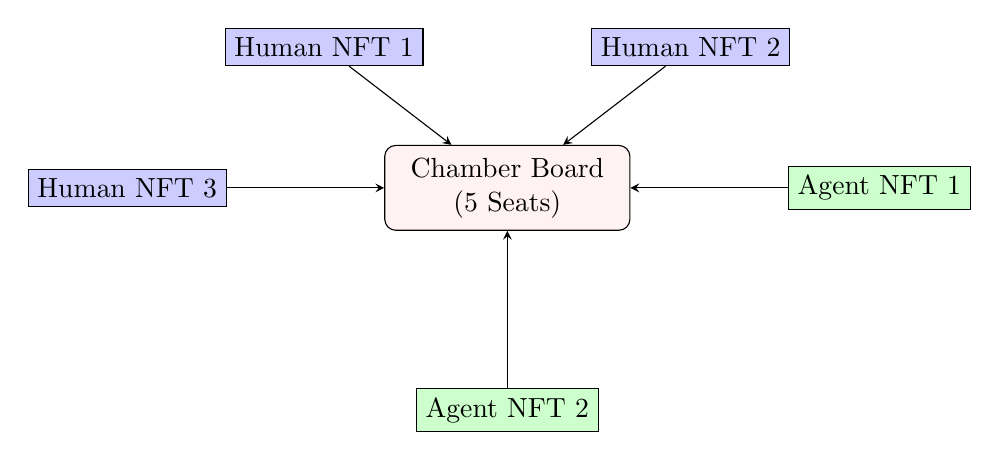
\begin{tikzpicture}[
    node distance=1.5cm,
    chamber/.style={draw,fill=pink!20,rounded corners,minimum width=2cm},
    nft/.style={draw,fill=blue!20,minimum width=1.5cm},
    agent/.style={draw,fill=green!20,minimum width=1.5cm}
]
    % Chamber in center
    \node[chamber] (C) {\begin{tabular}{c}Chamber Board\\(5 Seats)\end{tabular}};
    
    % Human NFT Holders
    \node[nft] (H1) [above left=1cm and -0.5cm of C] {Human NFT 1};
    \node[nft] (H2) [above right=1cm and -0.5cm of C] {Human NFT 2};
    \node[nft] (H3) [left=2cm of C] {Human NFT 3};
    
    % Agent NFT Holders
    \node[agent] (A1) [right=2cm of C] {Agent NFT 1};
    \node[agent] (A2) [below=2cm of C] {Agent NFT 2};
    
    % Draw connections to show board seats
    \draw[-stealth] (H1) -- (C);
    \draw[-stealth] (H2) -- (C);
    \draw[-stealth] (H3) -- (C);
    \draw[-stealth] (A1) -- (C);
    \draw[-stealth] (A2) -- (C);
\end{tikzpicture}
\caption{Chamber Board with Human and AI Agent NFT Holders}
\label{fig:chamber-hierarchy}
\end{figure}

The system supports the creation and management of SubDAOs that can operate with varying degrees of autonomy while maintaining connection to the parent Chamber. As illustrated in Figure \ref{fig:chamber-hierarchy}, each SubDAO Chamber maintains its own treasury and AI agents while inheriting governance parameters from the parent Chamber. Cross-Chamber coordination mechanisms enable complex multi-entity governance arrangements while maintaining clear lines of authority and responsibility.

\section{Use Cases}

\subsection{Treasury Management}
AI agents perform continuous analysis of market conditions, risk parameters, and investment opportunities. They generate detailed reports and recommendations while human leaders maintain strategic oversight and final decision-making authority. This hybrid approach combines the analytical capabilities of AI with human judgment and experience.

\subsection{Automated Governance}
The system enables automation of routine governance decisions within carefully defined parameters. This includes regular maintenance tasks, standard token distributions, and predictable operational decisions. The automation reduces administrative overhead while maintaining security through predefined constraints and human oversight.

\subsection{Hybrid Decision Making}
Complex governance decisions benefit from seamless collaboration between human leaders and AI agents. The agents provide data analysis, scenario modeling, and risk assessment, while human leaders contribute strategic insight, ethical considerations, and final approval. This creates a powerful synthesis of computational and human intelligence.

\section{Technical Implementation}

\subsection{Governance Contracts}
\begin{itemize}
    \item Membership NFT: \texttt{0xB99DEdbDe082B8Be86f06449f2fC7b9FED044E15}
    \item Governance Token: \texttt{0x7756d245527f5f8925a537be509bf54feb2fdc99}
    \item Team Multisig: \texttt{0x5d45a213b2b6259f0b3c116a8907b56ab5e22095}
\end{itemize}

\section{Conclusion}
Loreum embeds AI capabilities into traditional governance structures. The system's flexible architecture and robust safety mechanisms provide a foundation for more efficient and responsive organizational governance.

\end{document}